\documentclass[review]{elsarticle}

\usepackage{graphics, float, url}
\usepackage{graphicx}
\usepackage{subcaption}
\usepackage{lineno,hyperref}
\usepackage{mathtools}
\usepackage{multirow}
\usepackage{adjustbox}
\usepackage{chngpage}
\usepackage{setspace}
\usepackage{amsfonts}
\usepackage{subcaption}
\usepackage{float}
\usepackage[ruled, lined, onelanguage, linesnumbered]{algorithm2e}
\usepackage[usenames,dvipsnames,svgnames,table]{xcolor}
\newcommand{\myfloatalign}{\centering}
\modulolinenumbers[5]

\usepackage{epstopdf}
\epstopdfDeclareGraphicsRule{.tiff}{png}{.png}{convert #1 \OutputFile}
\AppendGraphicsExtensions{.tiff}

\journal{Applied Soft Computing}

%%%%%%%%%%%%%%%%%%%%%%%
%% Elsevier bibliography styles
%%%%%%%%%%%%%%%%%%%%%%%
%% To change the style, put a % in front of the second line of the current style and
%% remove the % from the second line of the style you would like to use.
%%%%%%%%%%%%%%%%%%%%%%%

%% Numbered
%\bibliographystyle{model1-num-names}

%% Numbered without titles
%\bibliographystyle{model1a-num-names}

%% Harvard
%\bibliographystyle{model2-names.bst}\biboptions{authoryear}

%% Vancouver numbered
%\usepackage{numcompress}\bibliographystyle{model3-num-names}

%% Vancouver name/year
%\usepackage{numcompress}\bibliographystyle{model4-names}\biboptions{authoryear}

%% APA style
%\bibliographystyle{model5-names}\biboptions{authoryear}

%% AMA style
%\usepackage{numcompress}\bibliographystyle{model6-num-names}

%% `Elsevier LaTeX' style
\bibliographystyle{elsarticle-num}
%%%%%%%%%%%%%%%%%%%%%%%
\newtheorem{definition}{Definition}
\begin{document}

\begin{frontmatter}

\title{Enhancing instance-level constrained clustering through differential evolution}

\author[mymainaddress]{Germ\'an Gonz\'alez-Almagro\corref{mycorrespondingauthor}}
\cortext[mycorrespondingauthor]{Corresponding author}
\ead{germangalmagro@ugr.es}

\author[mymainaddress]{Juli\'an Luengo}

\author[mysecondaddress]{Jos\'e-Ram\'on Cano}

\author[mymainaddress]{Salvador Garc\'ia}

\address[mymainaddress]{DaSCI Andalusian Institute of Data Science and Computational Intelligence, University of Granada, Spain}

\address[mysecondaddress]{Dept. of Computer Science, EPS of Linares, University of Ja\'en, Campus Cient\'ifico Tecnol\'ogico de Linares, Cintur\'on Sur S/N, Linares 23700, Ja\'en, Spain}

\begin{abstract}
Clustering has always been a powerful tool in knowledge discovery. Traditionally unsupervised, it received renewed attention when it was shown to produce better results when provided with new types of information, thus leading to a new kind of semi-supervised learning. This new information can be given in form of instance-level must-link and cannot-link constraints, in which this paper focuses on. We propose the first application of Differential Evolution to the constrained clustering problem, which is a generalization of traditional clustering that considers additional information in the form of constraints. We will compare the results obtained by this proposal to those obtained by previous nature-inspired techniques and by some of the state-of-the-art algorithms on 25 datasets with incremental levels of constraint-based information, supporting our conclusions with the aid of Bayesian statistical tests.
\end{abstract}

\begin{keyword}
constrained clustering, instance-level, must-link, cannot-link, genetic algorithm, differential evolution, Bayesian statistical tests.
\end{keyword}

\end{frontmatter}

\linenumbers

\section{Introduction} \label{sec:Intro}

One of the most widely known and studied data analysis problems is clustering. It is one of the most successful methods in the field of unsupervised learning, where there is no supervision on how the information should be handled. Clustering has been able to provide solutions in a large number of knowledge fields, such as, marketing, banking, psychology, psychiatry, astronomy, archaeology, genetics, cartographic labeling and image segmentation among others \cite{Everitt:2009:CA:1538772, araujo2019improving, verma2016improved, aparajeeta2016modified, wang2018non}.

In the literature, clustering methods are often divided into two subsets: partitional clustering and hierarchical clustering. The main difference is that in hierarchical clustering the result is not a partition of the data with a certain number of clusters---as in partitional clustering---, but instead a dendrogram in which there are partitions that include from the whole dataset to particular individuals \cite{Everitt:2009:CA:1538772}. A representative example of partitional clustering is the widely studied and well-known algorithm K-means, while for hierarchical clustering the CURE method should be highlighted \cite{wu2009top, guha1998cure}. In this paper we will focus on partitional clustering.

We can define partitional clustering as the task of grouping the instances of a dataset into $k$ clusters, so that new information can be extracted from them. A dataset $X$ is composed of $n$ instances, each one of them described by $d$ features. More formally, $X = \{x_1, \cdots, x_n\}$, with the $i$th instance noted as $x_i = (x_{[i,1]}, \cdots, x_{[i,d]})$. A typical clustering algorithm assigns a class label $l_i$ to each instance $x_i \in X$. As a result, we obtain the set of labels $L = \{l_1, \cdots, l_n\}$, with $l_i \in \{1, \cdots, k\}$, that effectively splits $X$ into $k$ non-overlapping clusters $c_i$ to form a partition called $C$. The criterion used to assign an instance to a given cluster is the similarity to the rest of elements in that cluster, and the dissimilarity to the rest of instances of the dataset, which can be obtained with some kind of distance measurement $d(\cdot, \cdot)$. An important detail is that each instance must belong to a single cluster \cite{jain1999data}. 

Semi-supervised learning (SSL) is a machine learning paradigm that arises from adding incomplete information to unsupervised learning. We can divide SSL methods into two broad categories according to their objective: semi-supervised classification and semi-supervised clustering. The first method has partial information about the labels, so it tries to minimize the error based on them while taking into account the distribution of unlabeled instances. The second tries to obtain better defined clusters incorporating background information to the clustering process, this is known as constrained clustering and is the main subject of the study presented in this paper \cite{chapelle2009semi, triguero2015self}. 

Constrained clustering is an SSL learning method whose goal is to find a partition of the dataset that meets the proper characteristics of a clustering method result, in addition to satisfying a certain constraint set. It has been successfully applied in many knowledge fields, among which it is worth mentioning: advanced robotics applications \cite{davidson2005clustering, semnani2016constrained}, applied marketing \cite{seret2014new}, obstructive sleep apnea analysis \cite{mai2018evolutionary}, handwritten digits classification \cite{li2015scalable}, Internet traffic classification \cite{wang2014internet}, electoral district designing, \cite{brieden2017constrained}, and lane finding in GPS data \cite{wagstaff2001constrained} among others.

Constraints can be understood in different ways, resulting in three main types of constrained clustering: cluster-level, instance-level and feature-level constrained clustering \cite{bradley2000constrained,davidson2007survey,schmidt2011clustering}. Moreover, hybrid approaches which try to integrate different types of constraints have also been proposed \cite{wang2010clustering}. 

In particular, we can find in the literature two types of instance-level constraints: pairwise constraints and distance-based constraints. In one hand, pairwise constraints tell us if two specific instances of a dataset must be placed in the same or in different clusters, resulting in Must-link (ML) and Cannot-link (CL) constraints respectively. On the other hand, distance-based constraints do not involve specific instances, but tell us if instances must be placed in the same or in different clusters based on a given distance measure \cite{davidson2007survey}. This paper focuses on pairwise instance-level constraints (ML and CL), which will be discussed later in Section \ref{sec:BackCC}.

Regarding the degree to which the constraints have to be satisfied, we can make a distinction between the concepts of hard and soft constraints. Hard constraints must necessarily be satisfied in the output partition of any algorithm that makes use of them, while soft constraints are taken as a strong guide for the algorithm that uses them but can be partially satisfied in the output partition \cite{seret2014new, wagstaff2001constrained, law2004clustering}. For the purposes of this paper, we will employ the latter.

Finding the optimal partition in a dataset, with respect to any kind of reasonable criteria, is known to be a $\mathbf{NP}$-hard problem. Therefore, the incorporation of constraints may modify the complexity of the clustering problem, depending on the type of constraints used. As we will study in more depth in Section \ref{sec:BackFeas}, the use of ML and CL constraints makes the constrained clustering problem $\mathbf{NP}$-complete \cite{davidson2005clustering}.

The constrained clustering problem can be formulated in terms of optimization, so that we can apply various optimization techniques to solve it. As mentioned earlier, it is a difficult problem to solve, so nature-inspired techniques are presented as a promising option to find quality approximate solutions. Nature is the best example of adaptive problem solving since it can apply an optimal strategy suited for each natural phenomenon \cite{fausto2019ants}. Nature-inspired algorithms are designed to emulate natural optimization phenomena, such as evolution, collective behavior of animals, physics laws or even human being-related processes. There have been attempts to solve the constrained clustering problem with nature-inspired algorithms, such as the adaptation of the Biased Random-key Genetic Algorithm (BRKGA) presented in \cite{de2017comparison}. Swarm-based methods have also been applied to constrained clustering, such as the one presented in \cite{xu2013improving}.

Differential Evolution (DE) is an evolution-based algorithm that has proven to be excellent in real-domain problem solving \cite{das2011differential}; in this paper we propose the first DE application to find quality solutions for the constrained clustering problem (see Section \ref{sec:SHADE}). In particular, we will take as basis for our proposal one of the DE variants which showed excellent behavior in worldwide competitions, known as SHADE \cite{molina2018insight}. We will make use of the Random-key concept from BRKGA, along with proposing a new fitness function, to build the already mentioned DE variant. We will properly compare the results obtained by our new method with previous nature-inspired algorithms, as well as with the constrained clustering state-of-the-art.

Regarding the organization of this paper, Section \ref{sec:background} reviews the existing knowledge concerning constrained clustering and DE. In Section \ref{sec:brkga} we will briefly review the BRKGA algorithm and its adaptation for constrained clustering. Afterward, the SHADE variant of DE algorithm will be presented in Section \ref{sec:SHADE}. In Section \ref{sec:SHADEadapt} we present the scheme that allow us to apply SHADE to constrained clustering, including the proposal of a new fitness function. Sections from \ref{sec:expSetup} to \ref{sec:analisis} present the experimental setup, results and their analysis respectively. Finally, in Section \ref{sec:conclusiones} we discuss conclusions.

\section{Background} \label{sec:background}

In this section we present the background knowledge concerning constrained clustering (Section \ref{sec:BackCC}), its computational complexity (Section \ref{sec:BackFeas}) and a brief description of some of the state-of-the-art methods for constrained clustering (Section \ref{sec:BackSOTA}). We will also present the basis of the DE optimization method (Section \ref{sec:BackDE}).

\subsection{Constrained Clustering} \label{sec:BackCC}

In most clustering applications it is common to have some kind of information about the dataset to be analyzed. In pairwise instance-level constrained clustering this information is given in the form of pairs of instances. A constraint states whether the instances which it refers to must, or must not, be assigned to the same cluster. It is possible to obtain a better result by using this type of information than by using completely unsupervised clustering algorithms. We can now formalize the two type of constraints mentioned: 

\begin{itemize}

	\item Must-link constraints $C_=(x_i,x_j)$: instances $x_i$ and $x_j$ from $X$ must be placed in the same cluster.

	\item Cannot-link constraints $C_{\neq}(x_i,x_j)$: instances $x_i$ and $x_j$ from $X$ cannot be assigned to the same cluster.

\end{itemize}

The goal of constrained clustering is to find a partition (or clustering) of $k$ clusters $C = \{c_1, \cdots, c_k\}$ of the dataset $X$ that ideally satisfies all constraints in the constraint set. As in the original clustering problem, it must be fulfilled that the sum of instances in each cluster $c_i$ is equal to the number of instances in $X$, which we have defined as $n = |X| = \sum_{i = 1}^{k} |c_i|$.

Knowing how a constraint is defined, ML constraints are an example of an equivalence relation; therefore, ML constraints are reflexive, transitive and symmetric. This way, given constraints $C_=(x_a,x_b)$ and $C_=(x_b,x_c)$ then $C_=(x_a,x_c)$ is verified. In addition, if $x_a \in c_i$ and $x_b \in c_j$ are related by $C_=(x_a,x_b)$, then $C_=(x_c,x_d)$ is verified for any $x_c \in c_i$ and $x_d \in c_j$ \cite{davidson2007survey}.

It can also be proven that CL constraints do not constitute an equivalence relation. However, analogously, given $x_a \in c_i$ and $x_b \in c_j$, and the constraint $C_{\neq}(x_a,x_b)$, then it is also true that $C_{\neq}(x_c,x_d)$ for any $x_c \in c_i$ and $x_d \in c_j$ \cite{davidson2007survey}.

\subsection{The Feasibility Problem} \label{sec:BackFeas}

Given that constrained clustering adds a new element to the clustering problem, we must consider how this element affects the complexity of the problem. The feasibility problem for non-hierarchical instance-level constrained clustering was defined in \cite{davidson2005clustering} as in Definition \ref{def1}.

\begin{definition}

	\textbf{Feasibility Problem}: given a dataset $X$, a constraint set $CS$, and the bounds on the number of clusters $k_l \leq k \leq k_u$, does there exist a partition $C$ of $X$ with $k$ clusters such that all constraints in $CS$ are satisfied? \cite{davidson2005clustering}
	\label{def1}

\end{definition}

In \cite{davidson2005clustering} it is proven that, when $k_l = 1$ and $k_u \ge 3$, the feasibility problem for constrained clustering is $\mathbf{NP}$-complete, by reducing it from the Graph K-Colorability problem (it is also proven that it is not harder, so both have the same complexity). Table \ref{tab:feasibility} shows the complexity of the feasibility for different types of constraints.

\begin{table}[!h]
	\centering
	%\setlength{\arrayrulewidth}{1mm}
	\setlength{\tabcolsep}{7pt}
	\renewcommand{\arraystretch}{1.2}
	%\resizebox{\textwidth}{!}{
		\begin{tabular}{c c}
			\hline
			Constraints & Complexity \\
			\hline
			Must-Link & $\mathbf{P}$\\
			Cannot-Link & $\mathbf{NP}$-complete\\
			ML and CL & $\mathbf{NP}$-complete\\
			\hline

		\end{tabular}%}
	\caption{Feasibility problem complexity \cite{davidson2005clustering}.}
	\label{tab:feasibility}
\end{table}

These complexity results show that the feasibility problem with CL constraints is intractable and hence constrained clustering is intractable too. For more details on the complexity of constrained clustering see \cite{davidson2005clustering}.

Intractable problems are hard to solve with deterministic and exact methods. That is the reason why nature-inspired algorithms constitute good approaches to find quality solutions to the constrained clustering problem.

\subsection{State-of-the-art Methods} \label{sec:BackSOTA}

Constrained clustering has many applications and has been widely studied in the literature. The first adaptation of a classic clustering method for constrained clustering was proposed in \cite{wagstaff2001constrained}. It involved modifying the widely studied K-means algorithm to take into account instance-level constraints: the already known ML and CL. This method was named COP-kmeans, it introduces a modification to the assignation rule of instances to clusters of the K-means algorithm so that an instance can be assigned to a cluster only if the assignment does not violate any constraint.

In \cite{antoine2012cecm} Constrained Evidential c-means (CECM), a variant of the Evidential c-means (ECM \cite{masson2008ecm}) algorithm is proposed, within the fuzzy clustering family of methods. The particularity of this algorithm is that the membership of instances to a cluster is defined by a probabilistic belief function. This method redefines constraints from the point of view of belief functions and includes them in the fitness function.

A modification of the Constrained Vector Quantization Error algorithm (CVQE \cite{davidson2005clustering}) is proposed in \cite{pelleg2007k}. The CVQE algorithm proved to produce high quality results, at the cost of a very high computational complexity. Linear CVQE (LCVQE) introduces a modification of the cost function of CVQE to make it more intuitive and less computationally complex. The experimentation resulted in a dramatic improvement of clustering quality over both noisy and clean constraint sets.

Two Views Clustering (TVClust) and Relation Dirichlet Process - Means (RDPM) were proposed in \cite{khashabi2015clustering}. TVClust is able to incorporate the constraints into the clustering problem by making a soft interpretation of them. The authors model the dataset and constraints in different ways, perform clustering methods on them and try to find a consensus between both interpretations. Using this model as a basis, the authors derive the deterministic algorithm RDP-means. This method can be viewed as an extension of K-means that includes side information (constraints) and has the property that the number of clusters ($k$) does not need to be specified.

\subsection{Short Introduction to Iterated Local Search}

Before defining the iterated local search---from now on ILS---,it is necessary to understand the local search and the motivation that leads to designing methods with greater exploratory capacity.

A local search is a procedure that consists of performing an heuristics-guided iterative improvement. Taking as initial state a well defined solution to the problem, the local search uses a neighbor generation operator to explore new solutions. When a solution better than the current one is found, it replaces the current one. In order to evaluate the solutions, the local search uses a function that assigns a value to each one of them, this is known as a target function. ***This value will be better the closer the solution that evaluates the optimal solution.*** 

Both the neighbor generation operator and the target function used by the local search must be defined for each problem. The target function $f(\cdot)$ determines how good the solution achieved is with respect to the purpose of the problem. The neighbor generation operator takes as base a solution to the problem $s$, and generates a new solution $s^\prime$ by modifying some of its components in a local way.

The Algorithm \ref{alg:LS} presents a basic scheme for a local search procedure. It is worth noting that the condition of line 4 must be adapted if the problem to be solved is one of maximization or minimization. In addition, the general scheme considers that the optimization process ends when the current solution is not improved, however the stop condition can be adapted to each problem.

\begin{algorithm}
	\SetNlSty{textbf}{[}{]}
	\SetNlSkip{0.5em}
	\setstretch{1.2}
	\SetKwFunction{GenerateNeighbor}{GenerateNeighbor}
	\SetKwRepeat{Do}{do}{while}
	\KwIn{Initial solution $s$}
	\BlankLine
	\While{$improvement$}{
		$improvement \leftarrow$ \texttt{false} \\
		
		$s^\prime \leftarrow $ \GenerateNeighbor{$s$}
		
		\If{$f(s^\prime) < f(s)$}{
			
			$s \leftarrow s^\prime$\\
			$improvement \leftarrow$ \texttt{true} \\
			
		}	
	}
	\BlankLine
	\KwRet ($s$)
	
	\caption{Local Search}\label{alg:LS}
\end{algorithm}

With the local search defined in this way, it is easy to see that the solution achieved will be the optimal local $s^*$ closest to the initial solution $s$. Figure \ref{img:LS} shows a pictorical representation of the above.

\begin{figure}[!h]
	\centering
	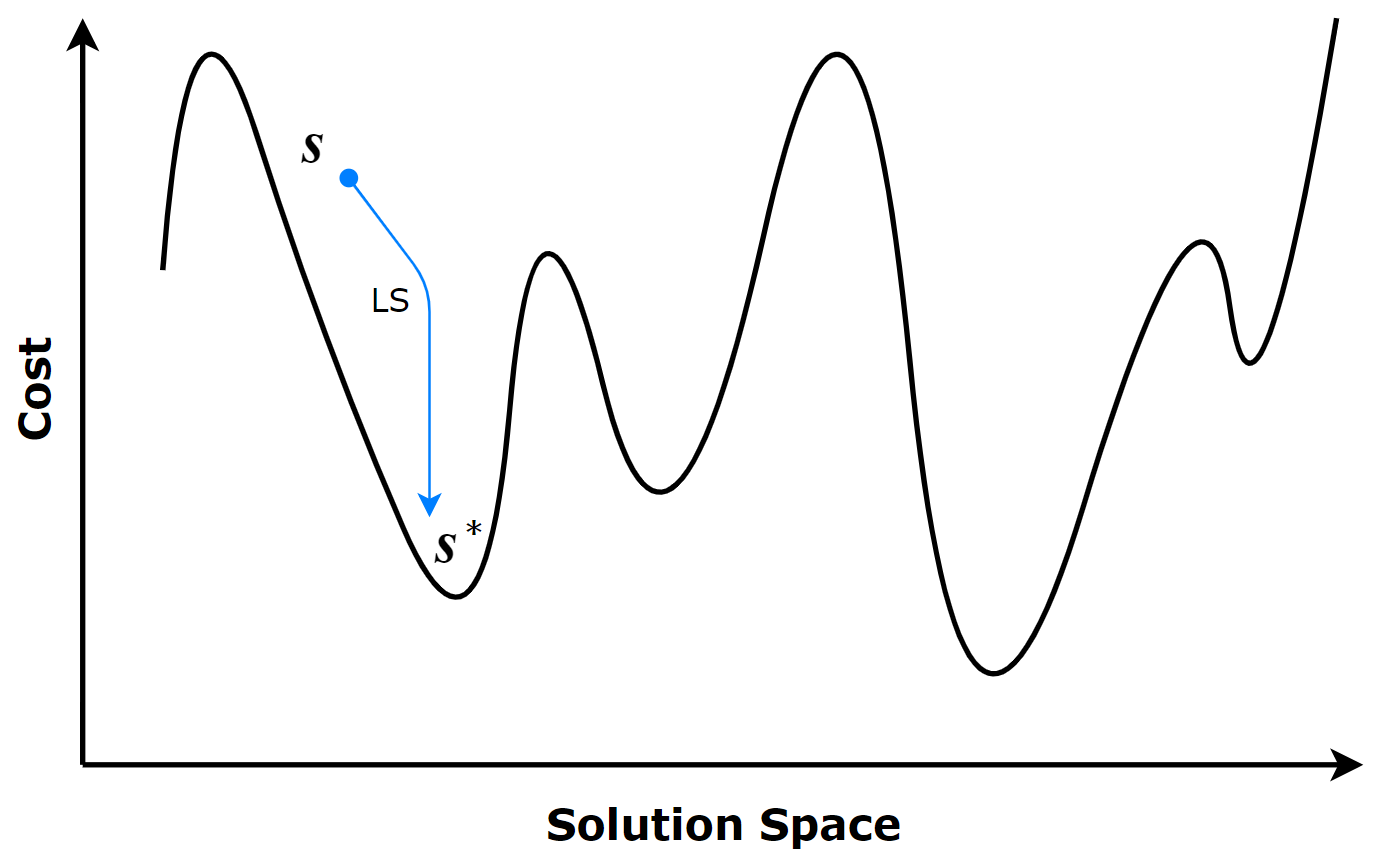
\includegraphics[scale=0.25]{Figures/LS.png}
	\caption{Local optimum achieved by a local search procedure}\label{img:LS}
\end{figure}

It is therefore necessary to appeal to techniques that introduce diversity in the search to avoid the problem of local optimal. This is exactly what ILS is trying to do.

With ILS, once we have reached a local optimum $s^*$, we apply a perturbation to it that, with a high probability, will result in a new solution $s^\prime$ that will not be a local optimum and will be far enough away from $s^*$. After that, we will apply a local search procedure to find a new local optimal $s^{*\prime}$. Figure \ref{img:ILS} shows a representation of the above concepts.

\begin{figure}[!h]
	\centering
	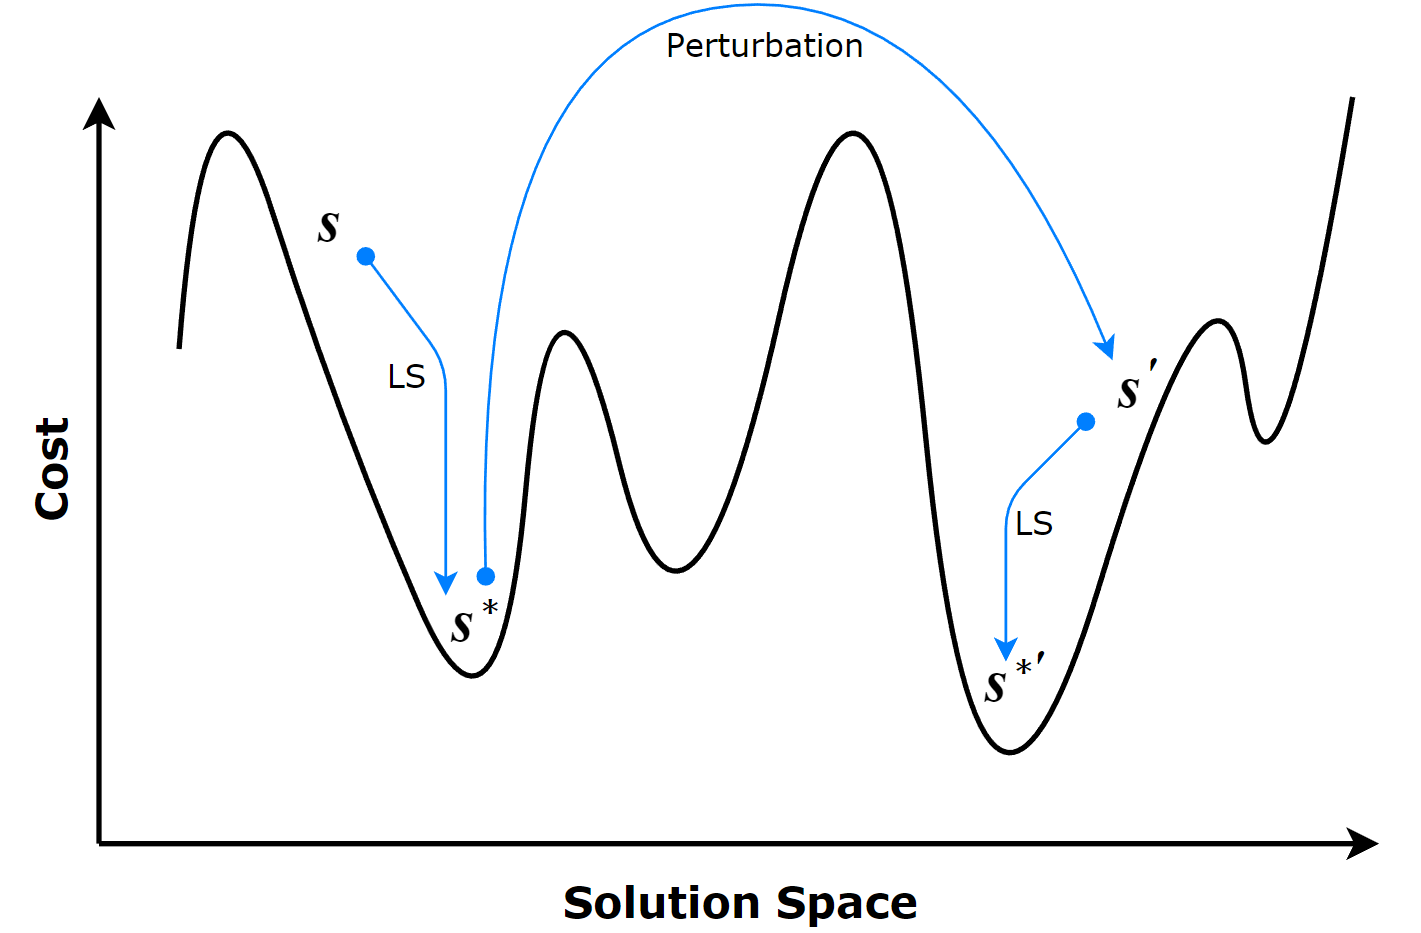
\includegraphics[scale=0.25]{Figures/ILS.png}
	\caption{No se como llamar a esta puta imagen}\label{img:ILS}
\end{figure}

It should be noted that, if the disturbance applied to $s*$ is too small, the most likely is that the local optimum closest to $s^\prime$ is $s^*$ and therefore the solution space will not be explored effectively. On the other hand, if the disturbance is too big, there will be no bias in the generation of new solutions, and therefore the procedure becomes a random reboot-type method.


The method for generating the perturbation applied to the local optimum $s^*$ may vary depending on the problem, and may be based on previous solutions. In this way, it is possible to keep a history of the solutions reached so far, so they can be used when applying the perturbation. Algorithm \ref{alg:ILS} summarizes the ILS overall optimization process.

\begin{algorithm}
	\SetNlSty{textbf}{[}{]}
	\SetNlSkip{0.5em}
	\setstretch{1.2}
	\SetKwFunction{LocalSearch}{LocalSearch}
	\SetKwFunction{Perturbation}{Perturbation}
	\SetKwRepeat{Do}{do}{while}
	\KwIn{Initial solution $s$}
	\BlankLine
	$s^* \leftarrow$ \LocalSearch{$s$}\\
	\While{Termination criteria are not met}{
		
		$s^\prime \leftarrow $ \Perturbation{$s^*$, $history$}\\
		$s^{*\prime} \leftarrow$ \LocalSearch{$s^\prime$}
		
		\If{$f(s^{*\prime}) < f(s^*)$}{
			
			$s^* \leftarrow s^{*\prime}$
			
		}	
	}
	\BlankLine
	\KwRet ($s*$)
	
	\caption{Iterated Local Search}\label{alg:ILS}
\end{algorithm}

In the ILS scheme described in Algorithm \ref{alg:ILS} the acceptance criterion only use the difference in the cost of the solutions to be compared to choose between them. This is the most simple scheme and does not depends on previous solutions recorded in the history.

\clearpage 

\section{The Dual Iterative Local Search Method}

\clearpage

\section{Experimental Setup} \label{sec:expSetup}

For our experiments we will compare the results obtained by BRKGA$_{CC}$ and SHADE$_{CC}$ over 25 datasets and 3 constraints set for each one of them. Most of these datasets can be found at the \href{https://sci2s.ugr.es/keel/category.php?cat=clas}{Keel-dataset repository} \cite{triguero2017keel}, though some of them have been obtained via
\href{https://scikit-learn.org/stable/datasets/index.html}{\texttt{scikit-learn} python package} \cite{scikit-learn}. We also include 3 artificial datasets in our analysis, namely: \textit{Circles}, \textit{Moons} and \textit{Spiral}, which can be found at GitHub. Table \ref{tab:datasets} displays a summary of every dataset.

\begin{table}[!h]
	\centering
	%\setlength{\arrayrulewidth}{1mm}
	%\setlength{\tabcolsep}{5pt}
	%\renewcommand{\arraystretch}{1.2}
	%\resizebox{\textwidth}{!}{
	\small
	\begin{tabular}{l c c c}
		\hline
		Name & No. Instances & No. Classes & No. Features \\
		\hline
		Appendicitis & 106 & 2 & 7 \\
		Breast Cancer & 569 & 2 & 30 \\
		Bupa & 345 & 2 & 6 \\
		Circles & 300 & 2 & 2 \\
		Ecoli & 336 & 8 & 7 \\
		Glass & 214 & 6 & 9 \\
		Haberman & 306 & 2 & 3 \\
		Hayesroth & 160 & 3 & 4 \\
		Heart & 270 & 2 & 13 \\
		Ionosphere & 351 & 2 & 33 \\
		Iris & 150 & 3 & 4 \\
		Led7Digit & 500 & 10 & 7 \\
		Monk2 & 432 & 2 & 6 \\
		Moons & 300 & 2 & 2 \\
		Movement Libras & 360 & 15 & 90 \\
		Newthyroid & 215 & 3 & 5 \\
		Saheart & 462 & 2 & 9 \\
		Sonar & 208 & 2 & 60 \\
		Soybean & 47 & 4 & 35 \\
		Spectfheart & 267 & 2 & 44 \\
		Spiral & 300 & 2 & 2 \\
		Tae & 151 & 3 & 5 \\
		Vowel & 990 & 11 & 13 \\
		Wine & 178 & 3 & 13 \\
		Zoo & 101 & 7 & 16 \\
		\hline

	\end{tabular}%}
	\caption{Summary of datasets used for the experiments.}
	\label{tab:datasets}
\end{table}

Classification datasets are commonly used in the literature to test constrained clustering algorithms; the reason behind this is that they enable us to generate constraints with respect to the true labels (see Section \ref{sec:ConstGent}). They also facilitate an easy evaluation of the quality of the algorithm by means of measures like the Adjusted Rand Index (see Section \ref{sec:EvalMet}).

\clearpage

\subsection{Constraint Generation} \label{sec:ConstGent}

Since we have the true labels associated with each dataset, we will use the method proposed in \cite{wagstaff2001constrained} to generate artificial constraint sets. This method consists of randomly selecting two instances of a dataset, then comparing its labels, and finally setting an ML or CL constraint depending on whether the labels are the same or different.

We will generate, for each dataset, three different sets of constraints---$CS_{10}$, $CS_{15}$ and $CS_{20}$---that will be associated with three small percentages of the size of the dataset: 10\%, 15\% and 20\%. With $n_f$ being the fraction of the size of the dataset associated with each of these percentages, the formula $\frac{n_f(n_f-1)}{2}$ tells us how many artificial constraints will be created for each constraint set; this number is equivalent to how many edges a complete graph with $n_f$ vertices would have.

The random allocation of constraints has a potential advantage over simply using the constraints contained in an $n_f$-vertex complete graph: there is a lower probability of biasing the constraint set towards having classes with poor representation in it. Table \ref{tab:constraints} shows the number of constraints of each type obtained for each dataset.

\begin{table}[!h]
	\centering
	\setlength{\tabcolsep}{7pt}
	\renewcommand{\arraystretch}{1.2}
	%\begin{adjustwidth}{-1in}{-1in}
	\resizebox{\textwidth}{!}{
	\begin{tabular}{lcc c cc c cc}
		\hline
		\multirow{2}{*}{Dataset} &
		\multicolumn{2}{c}{$CS_{10}$} && \multicolumn{2}{c}{$CS_{15}$} && \multicolumn{2}{c}{$CS_{20}$} \\
		\cline{2-3} \cline{5-6} \cline{8-9}
		& ML & CL && ML & CL && ML & CL \\
		\hline
		Appendicitis & 39 & 16 && 71 & 49 && 164 & 67 \\
		Breast Cancer & 876 & 720 && 1965 & 1690 && 3487 & 2954 \\
		Bupa & 323 & 272 && 699 & 627 && 1201 & 1145 \\
		Circles & 208 & 227 && 502 & 488 && 853 & 917 \\
		Ecoli & 163 & 398 && 357 & 918 && 609 & 1669 \\
		Glass & 52 & 179 && 139 & 389 && 259 & 644 \\
		Haberman & 304 & 161 && 634 & 401 && 1135 & 756 \\
		Hayesroth & 39 & 81 && 102 & 174 && 177 & 319 \\
		Heart & 178 & 173 && 396 & 424 && 744 & 687 \\
		Ionosphere & 330 & 300 && 732 & 646 && 1299 & 1186 \\
		Iris & 26 & 79 && 82 & 171 && 136 & 299 \\
		Led7Digit & 126 & 1099 && 267 & 2508 && 460 & 4490 \\
		Monk2 & 473 & 473 && 979 & 1101 && 1917 & 1824 \\
		Moons & 200 & 235 && 494 & 496 && 900 & 870 \\
		Movement Libras & 27 & 603 && 112 & 1319 && 158 & 2398 \\
		Newthyroid & 108 & 123 && 270 & 258 && 449 & 454 \\
		Saheart & 595 & 486 && 1292 & 1123 && 2330 & 1948 \\
		Sonar & 100 & 110 && 245 & 251 && 436 & 425 \\
		Soybean & 4 & 6 && 6 & 22 && 12 & 33 \\
		Spectfheart & 233 & 118 && 543 & 277 && 965 & 466 \\
		Spiral & 224 & 211 && 487 & 503 && 918 & 852 \\
		Tae & 40 & 80 && 82 & 171 && 151 & 314 \\
		Vowel & 445 & 4406 && 1026 & 10000 && 1705 & 17798 \\
		Wine & 49 & 104 && 121 & 230 && 217 & 413 \\
		Zoo & 21 & 34 && 29 & 91 && 41 & 169 \\
		\hline
		
	\end{tabular}}
	%\end{adjustwidth}

	\caption{Number of constraints used in experiments.}
	\label{tab:constraints}
\end{table}

Note that the greater the number of classes present in the dataset, the fewer ML constraints obtained with the method proposed in \cite{wagstaff2001constrained}. This is because the probability of randomly choosing two individuals from the same class decreases as the number of classes present in the dataset increases.

\clearpage

\subsection{Evaluation Method} \label{sec:EvalMet}

Since we have the true labels associated to each of the datasets, we can use them in post-processing to evaluate the results provided by each method. We will use the Adjusted Rand Index (ARI) to measure the accuracy of the predictions resulting from each method we test \cite{hubert1985comparing}. The basic Rand Index computes the degree of agreement between two partitions $C_1$ and $C_2$ of a given dataset $X$. $C_1$ and $C_2$ are viewed as collections of $n(n - 1)/2$ pairwise decisions \cite{rand1971objective}.

For each pair of instances $x_i$ and $x_j$ in $X$, a partition assigns them to the same cluster or to different clusters. We take $a$ as the number of pairings where $x_i$ is in the same cluster as $x_j$ in both $C_1$ and $C_2$, and $b$ as the opposite event ($x_i$ and $x_j$ are in different clusters in $C_1$ and $C_2$). Then, the degree of similarity between $C_1$ and $C_2$ is calculated as in Equation \eqref{eq15}.

\begin{equation}
\text{Rand}(C_1, C_2) = \frac{a + b}{n(n - 1)/2}
\label{eq15}
\end{equation}

The ARI is a corrected-for-chance version of the Rand Index. This correction uses the expected similarity of all comparisons between clusterings specified by a random model to set up a baseline. The ARI is computed as in Equation \eqref{eq16}.

\begin{equation}
\text{ARI}(C_1, C_2) = \frac{\text{Rand}(C_1, C_2) - \text{Expected Index}}{\text{Maximum Index} - \text{Expected Index}},
\label{eq16}
\end{equation}

\noindent where Maximum Index is expected to be 1 and Expected Index is the already mentioned expected degree of similarity with a random model. It is easy to see that $\text{ARI}(C_1, C_2) \in [-1,1]$, such that an ARI value close to 1 means a high degree of agreement between $C_1$ and $C_2$, a positive value close to 0 means no agreement and a value smaller that 0 means that the $\text{Rand}(C_1, C_2)$ is less than expected when comparing with random partitions. To summarize, the higher the ARI, the greater the degree of similarity between $C_1$ and $C_2$. For more details on ARI see \cite{hubert1985comparing}.

Our objective is to quantify the quality of the solutions obtained as a result of the methods presented in this paper. To accomplish this task we just set one of the two partitions given to compute ARI as the ground truth labels.

%% CORREGIR DESDE AQUI HASTA EL FINAL

\subsection{Calibration}

Table \ref{tab:params} shows a summary of the parameter setup used for both BRKGA$_{CC}$ and SHADE$_{CC}$ algorithms.

\begin{table}[!h]
	\centering
	\setlength{\tabcolsep}{7pt}
	\renewcommand{\arraystretch}{1.4}
	%\begin{adjustwidth}{-1in}{-1in}
	\resizebox{\textwidth}{!}{
		\begin{tabular}{>{\centering\arraybackslash}c m{5cm} cc}
			\hline
			Parameter & Meaning & BRKGA & SHADE \\
			\hline
			$|P|$ & Population size & 100 & 100 \\
			Evals & Fitness function evaluations & 300000 & 300000 \\
			$P_e$ & Size of the elite set in population & $0.2 * |P|$ & $0.25 * |P|$ \\
			$P_m$ & Number of mutants to be introduced in the population in each generation & $0.2 * |P|$ & - \\
			$p_\text{inherit}$ & Probability that a feature is inherited from an elite parent & $50\%$ & - \\
			$k$ & Output partition number of clusters & \multicolumn{2}{m{4cm}}{No. Classes (Table \ref{tab:datasets}).} \\
			\hline

		\end{tabular}}
		%\end{adjustwidth}

	\caption{Parameters setup used for BRKGA and SHADE.}
	\label{tab:params}
\end{table}

In both cases---BRKGA$_{CC}$ and SHADE$_{CC}$---the population size will be 100 individuals, and the stop criterion is given by the number of evaluations of the fitness function, which at most will be 300000.

To compare with the state-of-the-art methods mentioned in Section \ref{sec:BackSOTA} we will use the parameters setup shown in Table \ref{tab:paramsSOTA} for the implementation that can be found at \href{https://github.com/GermangUgr/TFG/tree/master/Software}{GitHub}

\begin{table}[!h]
	\centering
	\setlength{\tabcolsep}{7pt}
	\renewcommand{\arraystretch}{1.4}
	%\begin{adjustwidth}{-1in}{-1in}
	\resizebox{\textwidth}{!}{
		\begin{tabular}{>{\centering\arraybackslash}c m{5cm} c}
			\hline
			Common Parameters & Meaning & Value \\
			\hline
			\texttt{max\_iter} & Maximum number of iterations & 300 \\
			$k$ & Output partition number of clusters & No. Classes (Table \ref{tab:datasets}). \\
			\hline
			\hline
			Specific Parameters & \multicolumn{2}{l}{Name and Value} \\
			\hline
			COPKM & \multicolumn{2}{l}{\texttt{tolerance} = $1 * 10^{-4}$; \texttt{init\_mode} = \texttt{``rand''}} \\
			CECM & \multicolumn{2}{l}{$\alpha = 1$, $\rho = 100$, $\xi = 0.5$, \texttt{stop\_threshold} = $1 * 10^{-3}$, \texttt{init\_mode} = \texttt{``rand''}} \\
			LCVQE & \multicolumn{2}{l}{\texttt{initial\_centroids} = $\emptyset$} \\
			RDPM & \multicolumn{2}{l}{$\xi_0 = 0.1$, $\xi_\text{rate} = 1$, $\lambda$ is calculated on the basis of the mean distances in the dataset.} \\
			TVClust & \multicolumn{2}{l}{$\alpha_0 = 1.2$, \texttt{stop\_threshold} = $5*10^{-4}$} \\
			\hline
			
		\end{tabular}}
		%\end{adjustwidth}
		
	\caption{Parameters setup used for the state-of-the-art algorithms.}
	\label{tab:paramsSOTA}
\end{table}

Parameter values have been assigned following the guidelines of the original creators of the different proposals. Since the evaluation in the experimental stage makes use of a high number of datasets, tuning each parameter specifically for each dataset is not feasible. Indeed, our goal is not optimization in a case-by-case basis but instead a comparison in the most general scenario possible. Therefore, given that the purpose of this work is to draw a fair comparison between the algorithms and assess their robustness in a common environment with multiple datasets, we have not included a tuning step to maximize any particular performance metric.

\section{Experimental Results} \label{sec:results}

In this section we present Tables from \ref{tab:results10} to \ref{tab:results20SOTA}, which display the results obtained by the methods to be compared for each dataset and constraint set.

Since the methods we are comparing involve non-deterministic procedures, the results may vary from one run to another. To lessen the effect this may have on the results, we will apply each method 5 times to every dataset and constraint set, so that the measures shown in the previously mentioned tables correspond to the average of the 5 runs.

In this section we present a brief comparison between the proposed SHADE$_{CC}$ method and some of the state-of-the-art methods. Tables from \ref{tab:results10SOTA} to \ref{tab:results20SOTA} show the results obtained by these methods. To shorten the presented results this time we will only compare the ARI.

It should be noted that there are some missing results in these tables. In the case of the COPKM algorithm, this is due to the fact that it is highly dependent on the order in which constraints are analyzed. It is possible that COPKM cannot find a solution, even though it is always feasible, since the constraints have been generated based on the true labels. In the case of CECM, some of the results are not available because the memory structures that hold the algorithm grow non-linearly with the number of classes and the number of features of the dataset to be analyzed.
	
\begin{table}[!h]
	\centering
	\setlength{\tabcolsep}{7pt}
	\renewcommand{\arraystretch}{1.4}
	%\begin{adjustwidth}{-1in}{-1in}
	\resizebox{\textwidth}{!}{
		\begin{tabular}{lccccccc}
			\hline
			Dataset & DILS & BRKGA & COPKM & LCVQE & RDPM & TVClust & CEKM \\
			\hline
			Appendicitis & 0.611 & 0.022 & -1.000 & 0.335 & 0.316 & 0.025 & -0.005 \\
			Breast Cancer & 0.755 & 0.395 & -0.604 & 0.486 & 0.502 & 0.000 & 0.000 \\
			Bupa & 0.870 & 0.281 & -1.000 & -0.005 & -0.005 & -0.004 & -0.011 \\
			Circles & 0.798 & 0.166 & -1.000 & -0.003 & 0.162 & 0.137 & 0.133 \\
			Ecoli & 0.069 & 0.009 & -1.000 & 0.387 & 0.417 & 0.265 & -1.000 \\
			Glass & 0.009 & 0.016 & 0.184 & 0.268 & 0.197 & 0.211 & -1.000 \\
			Haberman & 0.638 & 0.047 & -1.000 & -0.002 & 0.127 & 0.218 & -0.004 \\
			Hayesroth & 0.031 & 0.027 & -1.000 & 0.106 & 0.097 & 0.054 & 0.139 \\
			Heart & 0.793 & 0.483 & -1.000 & 0.027 & 0.036 & 0.423 & -0.003 \\
			Ionosphere & 0.792 & 0.125 & -1.000 & 0.168 & 0.197 & 0.000 & 0.030 \\
			Iris & 0.621 & 0.238 & -0.285 & 0.730 & 0.607 & 0.244 & 0.684 \\
			Led7Digit & 0.016 & 0.009 & 0.497 & 0.425 & 0.369 & 0.316 & -1.000 \\
			Monk2 & 0.815 & 0.421 & 0.982 & 0.072 & 0.094 & -0.002 & 0.007 \\
			Moons & 0.968 & 0.277 & -1.000 & 0.241 & 0.319 & 0.785 & 0.092 \\
			Movement Libras & 0.022 & 0.004 & 0.285 & 0.293 & 0.256 & 0.000 & -1.000 \\
			Newthyroid & 0.028 & 0.017 & -1.000 & 0.579 & 0.289 & 0.846 & 0.002 \\
			Saheart & 0.800 & 0.147 & 0.974 & 0.018 & 0.020 & 0.068 & 0.000 \\
			Sonar & 0.649 & 0.124 & -1.000 & 0.004 & 0.013 & 0.000 & 0.000 \\
			Soybean & 0.304 & 0.496 & 0.503 & 0.545 & 0.621 & 0.000 & 0.244 \\
			Spectfheart & 0.896 & 0.334 & -1.000 & -0.107 & -0.114 & 0.000 & 0.050 \\
			Spiral & 0.856 & 0.058 & -1.000 & -0.003 & 0.012 & 0.034 & -0.002 \\
			Tae & 0.031 & 0.018 & -1.000 & 0.009 & -0.000 & 0.067 & 0.000 \\
			Vowel & 0.002 & 0.003 & -1.000 & 0.063 & -0.003 & 0.067 & -1.000 \\
			Wine & 0.334 & 0.120 & -1.000 & 0.360 & 0.368 & 0.281 & 0.004 \\
			Zoo & 0.151 & 0.105 & 0.715 & 0.666 & 0.412 & 0.335 & -1.000 \\
			\hline
			
		\end{tabular}}
		%\end{adjustwidth}
		
	\caption{Experimental results obtained for $CS_{10}$ comparing SHADE$_{CC}$ and the state-of-the-art.}
	\label{tab:results10SOTA}
\end{table}

\begin{table}[!h]
	\centering
	\setlength{\tabcolsep}{7pt}
	\renewcommand{\arraystretch}{1.4}
	%\begin{adjustwidth}{-1in}{-1in}
	\resizebox{\textwidth}{!}{
		\begin{tabular}{lccccccc}
			\hline
			Dataset & DILS & BRKGA & COPKM & LCVQE & RDPM & TVClust & CEKM \\
			\hline
			Appendicitis & 0.957 & 0.296 & -1.000 & 0.305 & 0.284 & 0.025 & -0.006 \\
			Breast Cancer & 0.788 & 0.772 & 1.000 & 0.486 & 0.502 & 0.000 & 0.037 \\
			Bupa & 0.984 & 0.840 & 1.000 & -0.005 & -0.007 & -0.007 & 0.001 \\
			Circles & 1.000 & 0.828 & 1.000 & -0.003 & 0.375 & 0.973 & 0.105 \\
			Ecoli & 0.134 & 0.015 & -1.000 & 0.387 & 0.372 & 0.719 & -1.000 \\
			Glass & 0.057 & 0.017 & -1.000 & 0.280 & 0.253 & 0.229 & -1.000 \\
			Haberman & 1.000 & 0.866 & 1.000 & -0.002 & 0.075 & 0.219 & -0.050 \\
			Hayesroth & 0.386 & 0.107 & -1.000 & 0.106 & 0.107 & 0.150 & 0.135 \\
			Heart & 1.000 & 0.692 & 1.000 & 0.025 & 0.033 & 0.442 & 0.000 \\
			Ionosphere & 0.970 & 0.803 & 1.000 & 0.178 & 0.212 & 0.000 & 0.057 \\
			Iris & 0.850 & 0.412 & -1.000 & 0.730 & 0.547 & 0.421 & 0.684 \\
			Led7Digit & 0.020 & 0.004 & -1.000 & 0.425 & 0.490 & 0.324 & -1.000 \\
			Monk2 & 0.902 & 0.751 & 1.000 & 0.072 & 0.170 & -0.002 & 0.007 \\
			Moons & 1.000 & 0.958 & 1.000 & 0.241 & 0.436 & 0.987 & 0.095 \\
			Movement Libras & 0.025 & 0.006 & -0.742 & 0.293 & 0.255 & 0.000 & -1.000 \\
			Newthyroid & 0.440 & 0.320 & -1.000 & 0.568 & 0.356 & 0.923 & 0.052 \\
			Saheart & 0.862 & 0.749 & 1.000 & 0.020 & 0.037 & 0.221 & 0.000 \\
			Sonar & 0.981 & 0.800 & -1.000 & 0.004 & 0.019 & 0.000 & 0.000 \\
			Soybean & 0.469 & 0.428 & 0.584 & 0.545 & 0.605 & 0.000 & 0.000 \\
			Spectfheart & 1.000 & 0.924 & 0.983 & -0.107 & -0.117 & 0.000 & -0.070 \\
			Spiral & 1.000 & 0.847 & -1.000 & -0.003 & 0.014 & 0.006 & 0.051 \\
			Tae & 0.299 & 0.119 & -1.000 & 0.008 & -0.004 & 0.062 & 0.000 \\
			Vowel & 0.003 & 0.002 & -1.000 & 0.063 & -0.003 & 0.073 & -1.000 \\
			Wine & 0.725 & 0.528 & -1.000 & 0.360 & 0.367 & 0.348 & -0.001 \\
			Zoo & 0.185 & 0.157 & 0.435 & 0.642 & 0.450 & 0.353 & -1.000 \\
			\hline
			
		\end{tabular}}
		%\end{adjustwidth}
		
		\caption{Experimental results obtained for $CS_{10}$ comparing SHADE$_{CC}$ and the state-of-the-art.}
		\label{tab:results15SOTA}
	\end{table}

\begin{table}[!h]
	\centering
	\setlength{\tabcolsep}{7pt}
	\renewcommand{\arraystretch}{1.4}
	%\begin{adjustwidth}{-1in}{-1in}
	\resizebox{\textwidth}{!}{
		\begin{tabular}{lccccccc}
			\hline
			Dataset & DILS & BRKGA & COPKM & LCVQE & RDPM & TVClust & CEKM \\
			\hline
			Appendicitis & 1.000 & 1.000 & -1.000 & 0.305 & 0.331 & 0.012 & -0.006 \\
			Breast Cancer & 0.807 & 0.807 & 1.000 & 0.486 & 0.502 & 0.000 & 0.000 \\
			Bupa & 0.991 & 0.936 & 1.000 & -0.005 & -0.007 & -0.006 & 0.000 \\
			Circles & 1.000 & 0.935 & 1.000 & -0.003 & 0.629 & 1.000 & 0.138 \\
			Ecoli & 0.201 & 0.028 & -1.000 & 0.387 & 0.459 & 0.763 & -1.000 \\
			Glass & 0.322 & 0.038 & -1.000 & 0.271 & 0.287 & 0.218 & -1.000 \\
			Haberman & 1.000 & 0.943 & 1.000 & -0.002 & 0.106 & 0.737 & 0.000 \\
			Hayesroth & 0.812 & 0.548 & -1.000 & 0.106 & 0.107 & 0.208 & 0.056 \\
			Heart & 1.000 & 0.942 & 1.000 & 0.025 & 0.033 & 1.000 & 0.000 \\
			Ionosphere & 0.982 & 0.902 & 1.000 & 0.173 & 0.309 & 0.000 & 0.115 \\
			Iris & 0.968 & 0.691 & -1.000 & 0.708 & 0.540 & 0.585 & 0.684 \\
			Led7Digit & 0.017 & 0.007 & -1.000 & 0.425 & 0.571 & 0.327 & -1.000 \\
			Monk2 & 0.904 & 0.855 & 1.000 & 0.072 & 0.253 & -0.002 & 0.160 \\
			Moons & 1.000 & 0.937 & 1.000 & 0.241 & 0.831 & 1.000 & 0.180 \\
			Movement Libras & 0.018 & 0.006 & -1.000 & 0.293 & 0.293 & 0.000 & -1.000 \\
			Newthyroid & 0.842 & 0.848 & -1.000 & 0.568 & 0.393 & 0.933 & 0.004 \\
			Saheart & 0.881 & 0.881 & 1.000 & 0.018 & 0.026 & 1.000 & -0.006 \\
			Sonar & 1.000 & 0.992 & 1.000 & 0.004 & 0.127 & 0.000 & 0.003 \\
			Soybean & 0.564 & 0.416 & -0.218 & 0.545 & 0.631 & 0.000 & -0.016 \\
			Spectfheart & 1.000 & 0.953 & 1.000 & -0.107 & -0.112 & 0.000 & -0.054 \\
			Spiral & 1.000 & 0.921 & 1.000 & -0.003 & 0.011 & 0.006 & 0.045 \\
			Tae & 0.892 & 0.351 & -1.000 & 0.008 & 0.000 & 0.035 & 0.000 \\
			Vowel & 0.003 & 0.002 & -1.000 & 0.063 & -0.003 & 0.071 & -1.000 \\
			Wine & 0.916 & 0.937 & -1.000 & 0.360 & 0.363 & 0.380 & 0.015 \\
			Zoo & 0.203 & 0.176 & 0.821 & 0.642 & 0.439 & 0.335 & -1.000 \\
			\hline
			
		\end{tabular}}
		%\end{adjustwidth}
		
		\caption{Experimental results obtained for $CS_{10}$ comparing SHADE$_{CC}$ and the state-of-the-art.}
		\label{tab:results25SOTA}
	\end{table}
	
	
\clearpage

\section{Statistical Analysis of Results} \label{sec:analisis}

With the results obtained by all methods for a total of 75 different datasets---the 25 datasets in combination with the 3 constraint sets for each one of them---we can perform an empirical analysis of them. This way we can statistically determine whether SHADE$_{CC}$ represents a significant improvement over previous proposals.

In order to carry out this study we will use Bayesian statistical tests, instead of the classic Hull Hypothesis Statistical Tests (NHST). In \cite{benavoli2017time} we find an in-depth analysis of the disadvantages of NHST, and a new model is proposed for carrying out comparisons researchers are interested in. \textit{"In a nutshell: NHST do not answer the question we ask"}. To put it clear, the disadvantages of the NHST that the authors highlight in \cite{benavoli2017time} are based on the trap of black-and-white thinking, this is: to reject, or not to reject?

To start with, NHST do not provide us with the probabilities associated to the analyzed hypotheses, and therefore it is not possible to answer the question: what is the probability that two methods are different? Another pitfall of NHST is that, with a sufficiently large number of observations, it is possible to reject almost any hypothesis. This is because the p-value does not allow us to separate between the effective size and the sample size, which is established by the researcher.

Also, NHST do not provide information about the magnitude of the effects and the uncertainty of its estimate. As a consequence, NHST may reject hypotheses despite very small effects, or even if there is significant uncertainty in the magnitude of the effects.

Furthermore, and this is a situation that all researchers have faced, NHST do not provide any information about the null hypothesis! That is: What can we conclude when NHST do not reject the null hypothesis? We can not infer anything since NHST can not provide evidence in its favor.

Finally, there are two other problems that researchers face when performing NHST. The first one is the choice of the significance level $\alpha$, for which there are no objective guidelines despite being critical to the test results. The second one is the need to previously formalize the intentions of the sampling of the results, which are usually fixed a posteriori; this could lead to a misreading of said results.

As shown in \cite{benavoli2017time}, most of these problems can be avoided by using Bayesian tests instead of NHST. In particular we will use the Bayesian sign test, which is the Bayesian version of the frequentist non-parametric sign test. To make use of it we will employ the R package \texttt{rNPBST}, whose documentation and guide can be found in \cite{carrasco2017rnpbst}.

From now on, and as far as the comparison of population-based methods is concerned, we will refer to the results obtained by BRKGA$_{CC}$ as sample $A$, and to the results obtained with SHADE$_{CC}$ as sample $B$.

The Bayesian sign test is based on obtaining the statistical distribution of a certain parameter $\rho$ according to the difference between the results, under the assumption that said distribution is a Dirichlet distribution. To get the distribution of $\rho$ we count the number of times that $A - B < 0$, the number of times where there are no significant differences, and the number of times that $A - B > 0$. In order to identify cases where there are no significant differences, we define the region of practical equivalence (rope) $[r_\text{min}, r_\text{max}]$, so that $P(A \approx B) = P(\rho \in \text{rope})$. Using these results we calculate the weights of the Dirichlet distribution and sample it to get a set of triplets with the following form: 
$$[P(\rho < r_\text{min}) = P(A - B < 0),\;\; P(\rho \in \text{rope}),\;\; P(\rho > r_\text{max}) = P(A - B > 0)]$$

One of the major advantages of the Bayesian sign test over the null hypothesis tests such as the (Wilcoxon's signed-rank test) is that we can obtain a visual representation of its results. We can produce a representation of the triplet set in the form of a heatmap where each triplet constitutes one point whose location is given by barycentric coordinates. With this in mind, we will associate each of the triplet values with each of the three vertices of an equilateral triangle. In order to find out where a certain triplet will be placed within the triangle, we will take each of its three values and draw a parallel line to the opposing side of the corresponding vertex; the separation between a triangle side and its parallel line will be proportional to the associated triplet value, so that the higher the value, the closer the line will be to the vertex. The location where the three lines intersect is where we draw a point. Since the values of every triplet describe a probability distribution and therefore they must add up to one, we can be sure that all triplets will lie in some point within the triangle. The color indicates the density of points in a given region, with yellow representing a high density and red a low density.

\begin{figure}[ht!]
	\centering
	\begin{subfigure}{.45\textwidth}
		\includegraphics[width=1\linewidth]{Figures/DILSvsBRKGA.pdf}
		\caption{ARI}
		\label{fig:DILSvsBRKGA}
	\end{subfigure}
	\begin{subfigure}{.45\textwidth}
		\includegraphics[width=1\linewidth]{Figures/DILSvsCOPKM.pdf}
		\caption{Time}
		\label{fig:DILSvsCOPKM}
	\end{subfigure}
	\begin{subfigure}{.45\textwidth}
		\includegraphics[width=1\linewidth]{Figures/DILSvsLCVQE.pdf}
		\caption{Unsat}
		\label{fig:DILSvsLCVQE}
	\end{subfigure}
	\begin{subfigure}{.45\textwidth}
		\includegraphics[width=1\linewidth]{Figures/DILSvsTVClust.pdf}
		\caption{Unsat}
		\label{fig:DILSvsTVClust}
	\end{subfigure}
	\begin{subfigure}{.45\textwidth}
		\includegraphics[width=1\linewidth]{Figures/DILSvsRDPM.pdf}
		\caption{Unsat}
		\label{fig:DILSvsRDPM}
	\end{subfigure}
	\begin{subfigure}{.45\textwidth}
		\includegraphics[width=1\linewidth]{Figures/DILSvsCEKM.pdf}
		\caption{Unsat}
		\label{fig:DILSvsCEKM}
	\end{subfigure}
	\caption{Heat diagrams.}
\end{figure}


\clearpage

\section{Conclusions} \label{sec:conclusiones}

In this paper we proposed SHADE$_{CC}$, the first application of a DE-based algorithm to the SSL constrained clustering problem. Focusing on the instance-level ML and CL constraints, SHADE$_{CC}$ has proven that nature-inspired evolution-based techniques constitute a good approach to constrained clustering, being able to scale the quality of the results in a way directly proportional to the number of constraints.
 
Supported by the Bayesian statistical tests, we were able to objectively prove that the SHADE$_{CC}$ approach is significantly better than previous evolution-based proposals. As far as the state-of-the-art is concerned, the SHADE$_{CC}$ approach has proven to be equivalent or better when considering the quality of the solutions, especially in cases where large sets of constraints are analyzed.

\section{Acknowledgements}

Our work has been supported by the research project TIN2017-89517-P and PP2016.PRI.I.02.

\clearpage

\section*{References}

\bibliography{mybibfile}

\end{document}